\section{结合深度学习的社交推荐}
传统的推荐算法存在一些固有缺点。基于邻域的方法虽然含义比较直观,具有比较高的可操作性,但是在用户和目标物体比较多时矩阵具有较高的稀疏性,而且采用矩阵的方式表示网络在需要增删操作时代价较高,以及冷启动的有效处理比较困难。而基于模型的算法,例如MF方法和二部图方法,虽然相较于基于邻域的方法有个更高的准确性和对用户、物品的关系进行了更深层的挖掘,但是仍然不能避免数据高稀疏的问题,冷启动同样是该类算法无法解决的问题之一。而当数据量变大时,会导致算法的运行效率下降,可解释性降低。


图与复杂网络这两种数据结构有着非常密切的关系,复杂网络可以看作为体量更大的图\cite{lu2011link}。将网络表示学习用于社交推荐的本质是基于用户产生的数据进行特征提取和相似度度量\cite{Ma2008SoRecSR}。而深度学习具有有效提取特征的能力,相较于传统的学习算法,深度学习算法通过更多的隐含数据特征提高了算法的准确度\cite{Singhl2017UseOD}.

\subsection{网络与深度学习的结合}

基于全连接的神经网络方法的基本思想来源于自然语言处理(Natural  Language Processing,NLP)中的词向量(Word Embedding,WE)成果。具体是指将随机游走得到的节点序列看作是自然语言处理中的句子,然后使用word2vec工具将节点转换成稠密的NE向量。应用比较广泛的有DeepWalk、node2vec 以及大规模信息网络表示学习方法(Large-scale Information Network Embedding,LINE)\cite{tang2015line}

基于简单神经网络的方法代表是DeepWalk算法\cite{Perozzi2014DeepWalkOL}.该算法是首个将深度学习技术与网络表示相结合的算法。它的基本思想借鉴了自然语言处理中生成词向量的方法\cite{Goldberg2014word2vecED}。具体过程是:首先通过随机游走算法的得到一段序列,然后使用Skip-gram 和Hierarchical Softmax \cite{mikolov2013efficient}模型对产生的序列中每个局部窗口中的节点进行概率建模,最后使用随机梯度下降算法进行参数的学习和更新。另一个比较典型的基于神经网络的算法是SDNE算法\cite{wang2016structural}。该算法利用深层神经网络对节点表示间的非线性进行建模。整个模型由两部分组成:一个是有特征矩阵建模的第一级相似度模块,另一个是由无监督的深层自编码器对第二级相似度关系进行建模。最终,SDNE 算法将深层自编码器的中间层作为节点的网络表示。 

在此基础上,有些研究者结合外部信息,例如文本信息、标签类别等,结合半监督学习的方法,对神经网络算法做了一些改进。node2vec 算法\cite{grover2016node2vec}对DeepWalk算法第一阶段的随机游走部分生成序列的方法进行了改造。DeepWalk u散发中随机游走序列产生新节点的方式是在均匀分布中随机抽样,而node2vec中则额外引入了两个参数,并通过广度优先搜索(Breadth First Search,BFS)和深度优先搜索(Depth First Search,DFS)来构造序列\cite{beamer2012direction} \cite{tarjan1972depth}。其中,获得最优超参数的方法,则采用网格搜索类半监督的学习。

相较于node2vec 和DeepWalk 这两种更看重节点与节点之间因连接而产生的隐含相互关系的方法,LINK算法同时加入了节点的二阶表示。所谓二阶标示就是将两个节点的共享邻居节点作为相关性的参考。具体而言,它是将一阶表示和二阶表示联合建模,通过最小化该模型的散度(Kullback–Leibler Divergence,KLD)\cite{van2014renyi}来求得向量的联合表示。这种算法显著提高了计算效率。

随着对各种非结构化数据的深入研究,越来越多的线性关系被发现,其中最著名的就是结构化深度网络表示学习(Structural Deep Network Embedding,SDNE)方法。该方法利用深度学习模型来捕获不同节点之间存在的线性关系,使用无监督编码器(Deep Auto Encoder,DAE)\cite{schmidhuber2015deep} 来对节点构成的二阶关系进行建模。直接使用一个拉普拉斯矩阵进行有监督的学习,录不同节点一阶的相
似度,联合 DAE 组成一个半监督学习结构。最终将 DAE 的中间隐含层作为输出,用来构建节点的稠密向量。 


\begin{table}[htbp]
    \centering 
    %{\begin{CJK*}{GBK}{hei}表X\quad 表说明 *表说明采用黑体*\end{CJK*}}
    \vspace {-2.5mm}
    \begin{center}
    \begin{tabular}{cccc}
    \toprule
    算法名& 优点& 缺点& 时间复杂度\\
    \hline
    DeepWalk& 效率较高& 隐关系挖掘不足& $O(d|V|log(|V|))$\\
    \hline
    node2vec& 效率较高& 隐关系挖掘不足& $O(d|V|)$\\
    \hline
    LINE& 效率极高& 隐关系挖掘不足& $O(d|E|)$\\
    \hline
    SDNE& 隐关系挖掘充分& 计算效率低& $O(d|V|^2)$\\
    \bottomrule
    \end{tabular}
    \label{tab1}
    \end{center}
    \end{table}

几种常见的深度学习与网络结合的算法对比如表\ref{tab1}所示。

\subsection{多层感知机}
利用推荐系统的社交关系可以缓解数据稀疏性问题,并有可能提高推荐性能。这种基于社会的推荐系统的开发是基于用户通常通过其最近的邻居用户获取和传播信息的现象。然而,大多数传统方法使用线性组合来处理社会特征,这可能导致在从社会关系中学习非线性特征时无效。DeepSoR\cite{fan2018deep} 提出了一种基于社会关系的深度神经网络模型。

\begin{figure}
    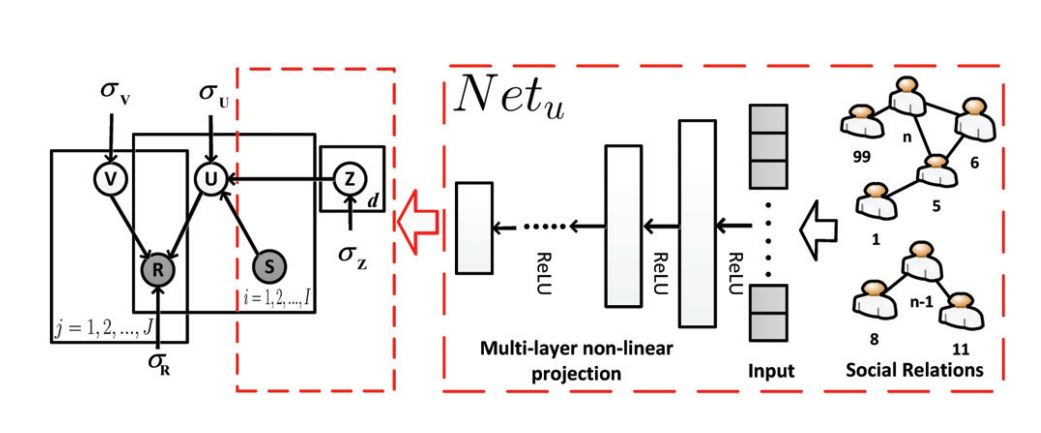
\includegraphics[width=0.9\linewidth]{dpfig/fig1.JPG}
    \caption{DeepSoR 系统框架}
    \label{fig1}
\end{figure}

该模型的系统框图如图\ref{1}所示。假设存在$I$ 个用户、$J$ 个项目和一个评价矩阵$R \in R^{I \times J}$。该网络的目标是找到用户和项目的潜在模型$U$ 和$V$ ,其乘积$U^TV$ 能够重构评价矩阵。可将观察到的等级上的条件分布定义为:

\begin{equation}
    p(R|U,V,\sigma_R^2) = \prod_i^I \prod_j^J N(r_{ij}|u_i^Tv_j, \sigma_R^2)^{c_{ij}}
\end{equation}

其中$N$表示高斯正态分布的概率密度函数。

通过用DNN(Netu)替换概率矩阵分解(PMF),模型中的用户潜在特征向量$u$由DNN生成的社会潜在向量来近似:

\begin{equation}
    u_i = Net_u(Z,s_i)+\epsilon_i 
\end{equation}

其中$s_i$是用户$i$的社交信息。定义给定Z和S的U的条件分布,以对用户潜在模型进行建模,如下所示:

\begin{equation}
    p(U|Z,S,\sigma_U^2) = \prod_i^I N(u_i|Net_u(Z,s_i),\sigma_U^2I)
\end{equation}

该模型在社交网络中采用最新的特征表示技术node2vec,旨在从用户的社交关系中学习用户到低维特征向量的映射。用户嵌入特征是node2vec根据用户$i$的社交关系生成的$q$维向量。此外,用户的偏好与在线社交网络中最近的邻居用户相似或受其影响。因此,人们采用了kNN技术来构成用户的邻居。使用基于用户嵌入功能的欧几里得距离,为每个用户返回k个最相似的邻居。然后,将与用户$i$的$k$个相似邻居相关的嵌入向量的平均值取为:$s_i=\sum \frac{e_a}{k}$。最后,将平均的嵌入向量$s_i$作为输入输入到非线性多层网络(隐藏层)中。

实验结果表明,该方法优于目前最先进的社会化推荐系统。

\subsection{循环神经网络(RNN)}
许多深层社交推荐器系统促进了社交网络信息以增强推荐性能,但是它们并未充分利用社交网络信息。首先,许多方法仅涉及直接邻居,而距离用户仅几步之遥的信息也可能会有所帮助。原因如下:1)信息通过社交网络传播,用户可能会受到间接邻居的影响; 2)当直接邻居无法共享有用的信息时,用户可能与远​​邻(或关系薄弱的邻居)产生联系。其次,大多数上述方法在所有推荐情况下均会平等对待邻居的信息。但是,当推荐器系统执行特定推荐时,并非来自邻居的所有信息都是有用的。例如,当预测用户是否将购买iPhone时,他/她的朋友与iPhone或其他与iPhone相关的物品之间的交互可能会有所帮助,而他/她的朋友与Nike鞋子之间的交互可能并不相关。因此,有必要过滤邻居的信息。最后,大多数深度社交推荐系统不会考虑用户对项目的意见,这些意见通常以评论或评分的形式表达出来。显而易见,用户朋友的好和坏意见会以极大不同的方式影响用户的决策。因此,需要仔细考虑用户-项目交互的观点。基于此,提出了以下深度神经网络模型DSCF\cite{fan2019deep},用以捕捉带有不同观点的社交信息。该网络的系统框图如图\ref{fig2}所示。

\begin{figure}
    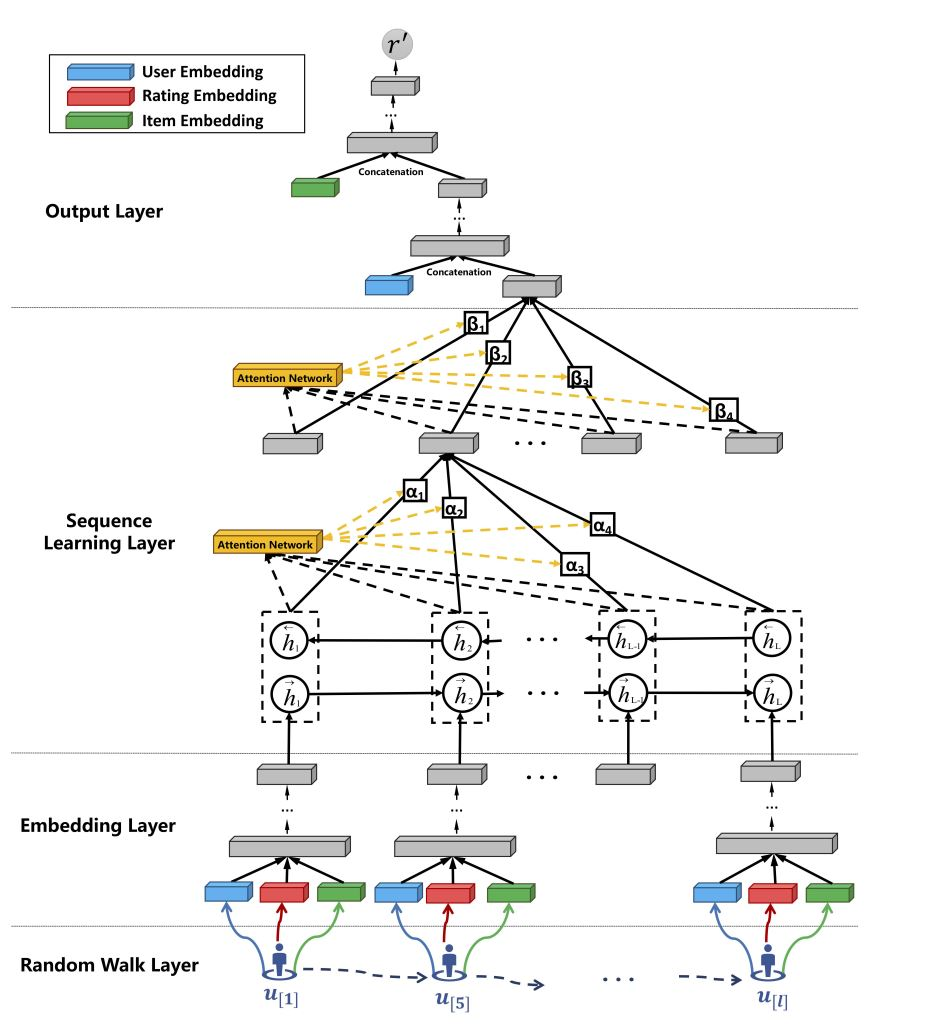
\includegraphics[width=0.9\linewidth]{dpfig/fig2.JPG}
    \caption{DSCF系统框架}
    \label{fig2}
\end{figure}

随机游走层:生成感知项目的社交序列。在社交推荐中,当我们尝试为给定用户$u$执行推荐时,不仅他/她的直接邻居可以提供有用的信息,而且在几跳之内的他/她的远近邻居(或他/她本地邻居中的邻居)也可以提供有用的信息。此外,与用户$u$距离不同的邻居可能对推荐的重要性不同。因此,在将$u$包括在用户$u$中作为推荐对象时,也有必要根据与用户$u$的距离来区分$u$的邻居。另外,随机游走以节点序列(用户序列)的形式探索邻居关系,自然而然地根据与用户$u$的距离保持邻居的顺序。因此,我们可以有效地利用随机游走从社交网络生成遥远的用户序列。

嵌入层:对用户-项目交互进行建模。项感知序列由来自用户邻居的用户项交互组成,因此,需要首先对用户项交互进行建模。在对用户-项目交互进行建模时,仔细考虑用户对交互表达的意见非常重要。显然,用户的社交邻居的好和坏意见会以极大不同的方式影响用户对项目的看法。因此,该模型建议在对序列中的用户与项目互动进行建模时,将用户对项目的意见包括在内。

序列学习层:用于项目感知社交序列的学习表示。序列学习层旨在提取每个序列的特征,然后结合所有序列的提取特征以获得未固定的表示形式,可用于预测输出层中$(u,v)$的等级。,对于遥远的邻居,我们需要捕获他们与用户$u$之间的遥信信息。此外,在社交网络中,用户相互影响。因此,我们需要捕获模型中的双向影响。近来,已经提出了基于双向长短期记忆网络(Bi-LSTM)的语言模型,以捕获NLP域中句子之间单词之间的双向双向语义依赖。受这些模型的启发,我们将序列视为“句子”,并将该序列中的元素视为“单词”,并采用类似的Bi-LSTM模型从融合的交互嵌入序列中提取特征。

该方法可以从遥远的社会关系中提取有用的信息以进行推荐,引入了一种在建模用户-项目交互时捕获用户意见的新颖方法,提出了一种可以充分利用社交网络信息的深层社会协作筛选框架。

\subsection{图卷积网络(GCN)}
\begin{figure}
    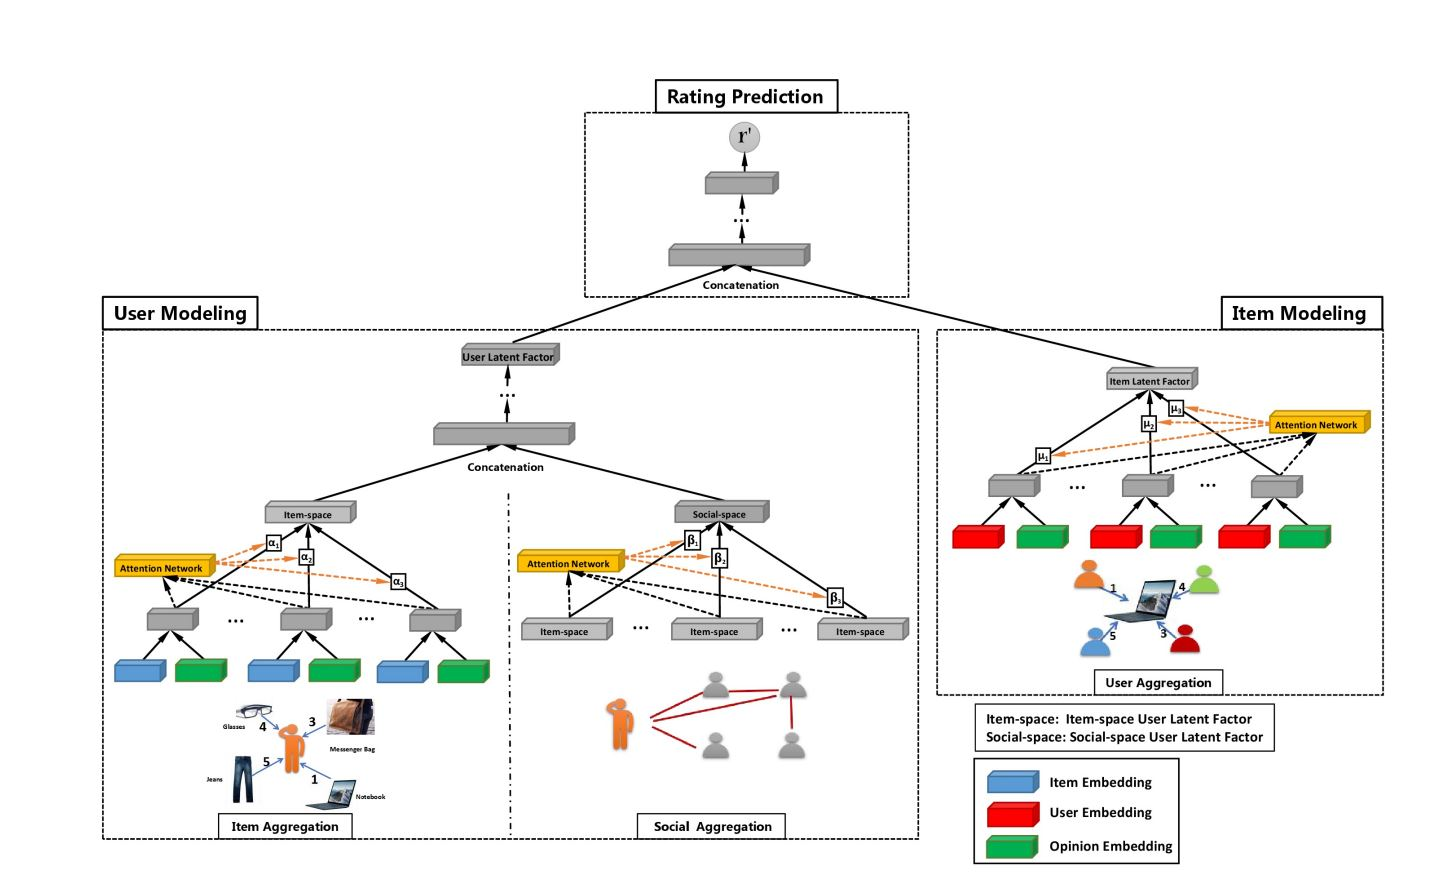
\includegraphics[width=0.9\linewidth]{dpfig/fig3.JPG}
    \caption{GraphRe框架}
    \label{fig3}
\end{figure}
事实证明,社会关系的引入有助于提高推荐效果。近年来,深度神经网络技术已用于图形数据。这些深层神经网络架构被称为图形神经网络(GNN)已。它们的主要思想是如何使用神经网络迭代地聚合来自局部图邻域的特征信息。同时,节点信息可以在变换和聚合之后通过图传播。因此,GNN自然地集成了节点信息以及拓扑结构,并已被证明在表示学习中很强大。另一方面,社交推荐中的数据可以表示为具有两个图形的图形数据。此外,社交推荐的自然方法是将社交网络信息整合到用户和潜在因素学习中。学习项目和用户的表示形式是构建社交推荐系统的关键。因此,鉴于其优势,GNN为推进社会推荐提供了前所未有的机会。比较典型的图卷积网络为GraphRe\cite{fan2019graph}。该网络的系统框图如图\ref{fig3}所示。


该模型由三个部分组成:用户建模,项目建模和评级预测。第一个组件是用户建模,它是要学习用户的潜在因素。由于社交推荐系统中的数据包括两个不同的图,即社交图和用户项目图,因此有很大的机会从不同的角度学习用户表示。因此,引入了两个聚合来分别处理这两个不同的图。一种是项目聚合,可用于通过用户与用户项目图中的项目(或项目空间)之间的交互来了解用户。另一个是社交聚合,即社交图中用户之间的关系,可以帮助从社交角度(或社交空间)建模用户。然后,直观地通过组合来自项目空间和社交空间的信息来获取用户潜在因素。第二部分是项目建模,它是学习项目的潜在因素。为了在用户项目图中同时考虑交互和意见,我们引入了用户聚合,即聚合用户意见项目建模。第三个组件是通过集成用户和项目建模组件来通过预测学习模型参数。

该模型可以连贯地对社交推荐中的图数据进行建模;提供了一种原则性的方法来共同捕获用户项目图中的交互和观点;在各种现实世界的数据集上证明了该框架的有效性。 

\subsection{对抗神经网络}
大多数现有的社交推荐方法将用户表示用于用户-项目交互(项目域)和用户用户连接(社交域)。但是,由于用户在两个域中的行为和交互不同,这可能会限制每个相应域中的用户表示学习,这使他们的表示形式变得异构。另外,大多数传统的推荐系统无法有效地优化这些目标,因为它们采用了负采样技术,该技术无法在优化过程中为培训提供足够的信息性指导。DASO\cite{fan2019deep}提出了一种新颖的“深度对抗社会建议”。它采用双向映射ping方法,通过对抗学习在社交域和项目域之间传递用户信息。该系统的框图如图\ref{fig4}

\begin{figure}
    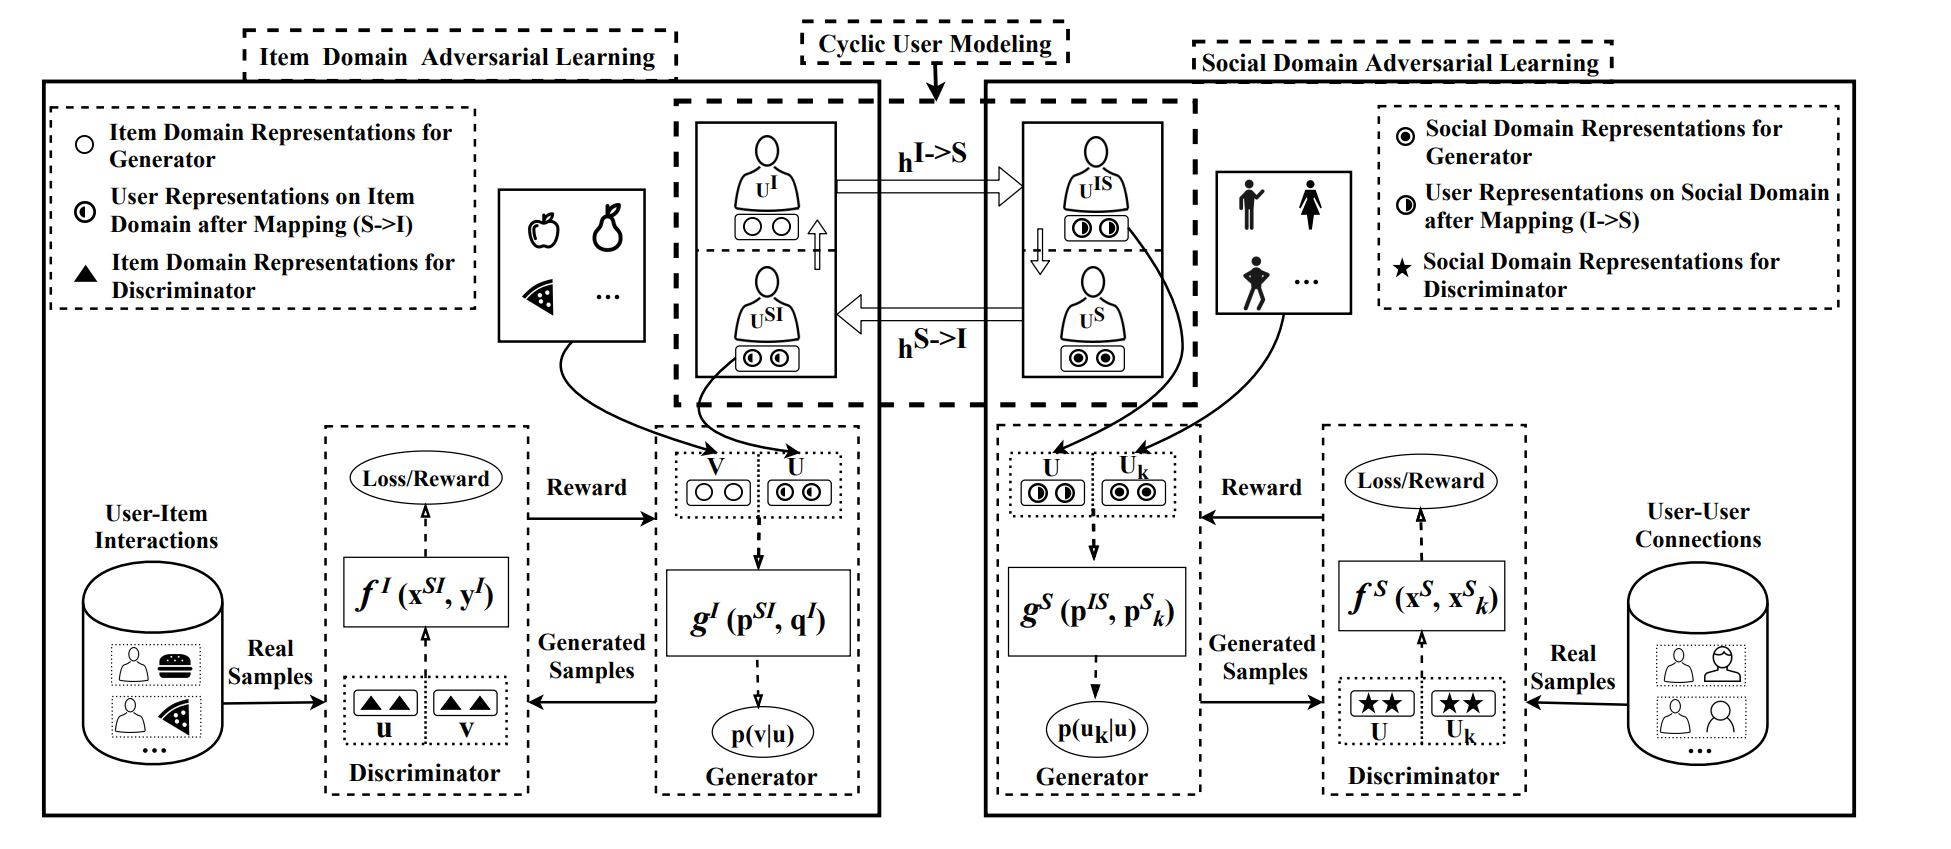
\includegraphics[width=0.9\linewidth]{dpfig/fig4.JPG}
    \caption{DASO系统框架}
    \label{fig4}
\end{figure} 

信息来自两个领域,分别是项目域$I$和社交域$S$。该模型由三个部分组成:循环用户建模,项目域对抗性学习和社交领域对抗性学习。其中,项目域对抗学习是采用对抗学习的方式来动态生成“困难”、信息量大的负样本来指导用户和项目的表示学习。生成器用于为每个用户“采样”(推荐)项目,并输出用户-项目对作为虚假样本;另一个是鉴别器,它将从真实的用户-项目交互对中区分生成的用户-项目对样本;社交域中的对抗学习与上述类似,也包括生成器和鉴别器,不同的是,其是从真实的用户-用户连接对中区分生成的"假"社交关系;循环用户建模组件旨在建模两种域中用户和项目的特征表示的联系。

该模型引入了一种使用双向映射方法将用户信息从社交域转移到商品域的原则方法,其中在两个域之间循环信息以逐步增强用户表示;提出了深度对抗性社交推荐器系统DASO可以利用对抗学习的力量动态生成“困难的”负样本,了解两个主体之间的双向映射,并最终优化更好的用户和物品表示。

\subsection{深度学习不适用的情形}

首先,在数据量偏小的情况下,并不适合应用深度学习。因为深度学习具有海量的参数需要训练,小的数据量容易出现过拟合的情况,降低模型对训练集以外样本的准确性。

其次,当数据不存在局部相关特性时,深度学习方法的表现也不好。深度学习之所以能在计算机视觉以及自然语言处理领域大放异彩,是因为图像和文本数据都具有局部相关性。比如图像中,相邻的点组成边,相连的边组成轮廓,可谓一个像素不能表达足够的信息,但一堆像素就能表示这是人脸还是狗头;语言中由单词组成句子,相邻的单词间存在相近的表达,同时单词间的次序一旦被打乱,那么整体所表达的信息也同时被打乱了。这些具有局部相关特性的数据,配合以特定的网络结构可以提取出其中的局部相关特性,同时配合深度架构达到层次特征的提取,从而达到令人满意的效果。而对于不具有局部相关特性的数据,没法用特定的网络拓扑来捕捉它们的信息,在深度学习中就只能用MLP来完成模型的训练,而通常MLP的效果通常要弱于GDBT , RF等传统集成树模型。

再者,不同的数据形式需要设计特定的网络结构,不存在通用的深度学习架构。图像数据被表示为二维矩阵的形式(当然三通道的图像被表示为三维矩阵),为了获取图像的局部特征,人们基于平移不变性设计出了参数共享的卷积神经网络(CNN),利用滑动窗口可以很好的捕捉局部特征,并且缩小了参数空间;文本数据被表示为序列的形式,人们基于分布式假设设计出了带滑动窗口的词嵌入技术(Word2vec),使得学到的词向量具有推理的作用;对于带有时间序列的数据,人们设计出了循环神经网络(RNN),使得参数可以受上一时刻的影响;对于图结构的数据,最近人们又设计出了图卷积神经网络(GCN)来更好的获取图结构上的特征;对于没有特殊形式的数据,深度学习不见得能更胜一筹,当人工特征工程做到一定程度后,传统模型是可以超越深度学习的。